% =====================================================================
%  EcoBin — Technical Report
%  Compile with: pdflatex EcoBin-Report.tex   (run twice for the ToC)
%  Only standard TeX Live / MiKTeX packages are used.
% =====================================================================
\documentclass[11pt,a4paper]{article}

\usepackage[utf8]{inputenc}
\usepackage[T1]{fontenc}
\usepackage{lmodern}
\usepackage{microtype}
\usepackage[margin=2.4cm]{geometry}
\usepackage{graphicx}
\usepackage{booktabs}
\usepackage{tabularx}
\usepackage{multirow}
\usepackage{xcolor}
\usepackage{tikz}
\usepackage{pgfplots}
\usepackage{amsmath}
\usepackage{enumitem}
\usepackage{fancyhdr}
\usepackage{caption}
\usepackage{textcomp}
\usepackage[hidelinks]{hyperref}

\usetikzlibrary{positioning,arrows.meta,calc,shapes.geometric,fit,backgrounds}
\pgfplotsset{compat=1.18}

% --- palette ---------------------------------------------------------
\definecolor{ink}{HTML}{10151C}
\definecolor{inksoft}{HTML}{4A5666}
\definecolor{accent}{HTML}{C2490A}
\definecolor{rule}{HTML}{DDE2EA}
\definecolor{wash}{HTML}{F5F7FA}
\definecolor{crit}{HTML}{E11D48}
\definecolor{high}{HTML}{EA7317}
\definecolor{med}{HTML}{C9930F}
\definecolor{low}{HTML}{0D9268}

\captionsetup{font=small,labelfont={bf,color=accent},skip=6pt}
\setlist[itemize]{leftmargin=1.3em,itemsep=2pt,topsep=4pt}
\setlist[enumerate]{leftmargin=1.6em,itemsep=2pt,topsep=4pt}

\pagestyle{fancy}
\fancyhf{}
\renewcommand{\headrulewidth}{0.4pt}
\fancyhead[L]{\small\textsc{EcoBin}}
\fancyhead[R]{\small\textsc{Technical Report}}
\fancyfoot[C]{\small\thepage}

\newcommand{\co}{CO\textsubscript{2}}
\newcommand{\num}[1]{\texttt{#1}}

% =====================================================================
\begin{document}

% ---------------------------------------------------------------- title
\begin{titlepage}
\centering
\vspace*{2.2cm}

{\color{accent}\rule{\textwidth}{1.4pt}}\\[0.7cm]

{\fontsize{46}{50}\selectfont\bfseries EcoBin}\\[0.5cm]

{\Large A demand-driven dispatch system for municipal waste collection}\\[0.35cm]

{\large\itshape Sensor-led ranking, fleet partitioning and route optimisation}\\[0.6cm]

{\color{accent}\rule{\textwidth}{1.4pt}}\\[1.6cm]

\begin{minipage}{0.82\textwidth}
\centering\large
Bins report how full they are. The system decides which ones matter,
splits the round across the available fleet, and routes each truck
the short way --- reducing driven distance by a measured
\textbf{33\,\%} against the order an operator would otherwise drive.
\end{minipage}

\vfill

\begin{tabular}{rl}
\textbf{Deployment} & Guwahati, Assam (pilot) \\[2pt]
\textbf{Telemetry}  & ThingSpeak \\[2pt]
\textbf{Routing}    & OpenRouteService, OSRM \\[2pt]
\textbf{Automation} & n8n, Firebase Firestore \\[2pt]
\textbf{Source}     & 8{,}441 lines across 37 files \\
\end{tabular}

\vspace{1.4cm}
{\small All figures in this report were produced by executing the system.\\
None are estimated.}

\vspace{1.2cm}
\end{titlepage}

% ---------------------------------------------------------------- toc
\tableofcontents
\newpage

% =====================================================================
\section{Abstract}

Municipal waste collection is normally scheduled rather than demanded. A
truck drives a fixed route on a fixed day, emptying bins that are a
quarter full and passing bins that overflowed two days earlier. The waste
is the visible failure; the fuel is the expensive one.

EcoBin replaces the schedule with a decision chain. Bins publish fill
level and weight to ThingSpeak. Each bin is scored on how urgently it
needs attention. Bins that need collecting are partitioned across the
available fleet by angular sector around the depot, each truck's stops
are ordered to minimise real driving time, and the resulting run is
dispatched --- automatically, if an external workflow requests it.

The contribution is not any single algorithm; all are established. It is
the composition: a scoring model that separates \emph{urgency} from
\emph{whether a truck is the right response}, a partitioning step that
searches its own starting angle, a tour optimiser that is provably never
worse than doing nothing, an emissions model that exposes its own
arithmetic, and a sensor-fusion rule that refuses to believe a load cell
reading zero while the bin is visibly full.

On a five-bin fleet against the real Guwahati road network, the planned
run is \textbf{14.83\,km} against a fullest-first baseline of
\textbf{22.10\,km} --- a \textbf{33\,\%} reduction, \textbf{2.60\,litres}
of diesel and \textbf{7.0\,kg} of \co{} per run.

% =====================================================================
\section{Problem statement}

\subsection{Why fill sensors alone are not a solution}

Instrumenting a bin is the easy part. A commodity ultrasonic sensor and a
load cell will tell you a bin is 84\,\% full and holding 71\,kg. That
information is close to useless on its own, because it answers none of
the three questions an operator actually faces each morning:

\begin{enumerate}
  \item Of the eleven bins reporting as full, which matters most?
  \item Which of the four available trucks should take which bins?
  \item In what order should each truck drive its stops?
\end{enumerate}

Question three is the one with the money in it. A refuse collection
vehicle manages roughly 2.5--3\,km per litre of diesel; it is heavy and
it stops constantly. Every unnecessary kilometre is approximately one
kilogram of \co{} and a measurable operating cost. A system that
identifies full bins but sequences them badly can easily drive further
than the fixed schedule it replaced.

\subsection{The failure mode this targets}

Consider a naive sensor-driven system that dispatches to the fullest bin
first. On a five-bin round it produces:

\begin{center}\small
\texttt{Depot $\rightarrow$ Station Rd $\rightarrow$ Market $\rightarrow$ Hospital $\rightarrow$ Terminus $\rightarrow$ Riverside $\rightarrow$ Depot}
\end{center}

This is a defensible-looking order that ignores geography entirely. The
truck crosses the city to reach the 96\,\% bin, then doubles back past
three others to reach the 94\,\% one. Measured on the real road network,
that route is 22.10\,km. The geographically optimised order over the same
five stops is 14.83\,km. The sensors were identical; only the decision
changed.

% =====================================================================
\section{System architecture}

The system is a five-stage chain. Each stage is independently testable,
and no stage requires an EcoBin-operated server: the dashboard compiles
to a static bundle.

\begin{figure}[h]
\centering
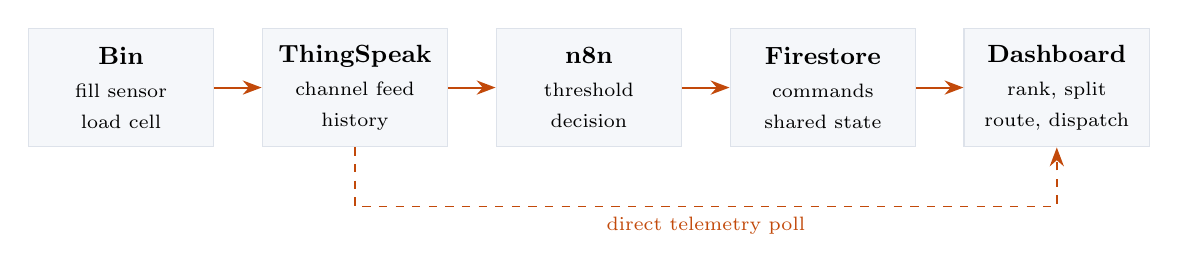
\begin{tikzpicture}[
  node distance=6mm,
  stage/.style={draw=rule,fill=wash,line width=0.6pt,minimum width=2.35cm,
                minimum height=1.5cm,align=center,font=\small},
  lbl/.style={font=\scriptsize\color{accent}},
  ar/.style={-{Stealth[length=2.4mm]},draw=accent,line width=0.7pt}
]
\node[stage] (a) {\textbf{Bin}\\[1pt]\scriptsize fill sensor\\\scriptsize load cell};
\node[stage,right=of a] (b) {\textbf{ThingSpeak}\\[1pt]\scriptsize channel feed\\\scriptsize history};
\node[stage,right=of b] (c) {\textbf{n8n}\\[1pt]\scriptsize threshold\\\scriptsize decision};
\node[stage,right=of c] (d) {\textbf{Firestore}\\[1pt]\scriptsize commands\\\scriptsize shared state};
\node[stage,right=of d] (e) {\textbf{Dashboard}\\[1pt]\scriptsize rank, split\\\scriptsize route, dispatch};

\draw[ar] (a) -- (b);
\draw[ar] (b) -- (c);
\draw[ar] (c) -- (d);
\draw[ar] (d) -- (e);

\draw[ar,dashed] (b.south) -- ++(0,-0.75) -| node[lbl,pos=0.25,below]{direct telemetry poll} (e.south);
\end{tikzpicture}
\caption{The dispatch chain. The dashed path is the dashboard's own
telemetry poll, independent of the automation branch --- the map stays
live whether or not n8n is running.}
\end{figure}

\subsection{Why the final hop is a subscription}

A browser page can initiate requests but cannot receive them. With no
server process holding a connection open, an inbound webhook URL for the
dashboard is not merely unimplemented but impossible.

Firestore resolves this correctly: n8n writes a command document, and the
dashboard --- already subscribed to that collection --- reacts within
approximately one second. Command claiming is transactional, so two
dashboards observing the same workspace cannot both dispatch a truck to
the same bin. A polling fallback against an n8n webhook exists for
deployments with no Firebase project, at the cost of poll-interval
latency and a CORS requirement on the workflow.

% =====================================================================
\section{Priority ranking}

\subsection{Model}

Each bin receives a score in $[0,100]$. Fill level provides the backbone,
scaled against the operator's configured thresholds rather than a
hard-coded constant. Seven further terms adjust it. Every term that fires
appends a human-readable reason, so the ranking can be argued with rather
than taken on faith.

\begin{table}[h]
\centering\small
\begin{tabularx}{\textwidth}{lrX}
\toprule
\textbf{Signal} & \textbf{Contribution} & \textbf{Rationale} \\
\midrule
Fill level             & $0 \rightarrow 80$ & Backbone; scaled to configured thresholds \\
Projected time to full & $+20$ & A fast-filling bin outranks a static fuller one \\
Open citizen report    & $+18$ & A person complained; that beats a clean sensor \\
Over capacity by weight& $+15$ & Load cell catches overflows the fill sensor misses \\
Silent / offline       & $+35$ & An unknown cannot be planned around \\
Battery below 20\,\%   & $+10$ & The bin is about to become an unknown \\
Days uncollected       & $+10$ & A slow bin still needs a visit eventually \\
\midrule
Truck already en route & $\times 0.25$ & Damper --- visible, but not outstanding work \\
Under maintenance      & cap at $15$ & Damper --- no longer a collection decision \\
\bottomrule
\end{tabularx}
\caption{Scoring terms. Dampers are applied after the additive terms.}
\end{table}

\subsection{Fill-rate extrapolation}

The time-to-full term is the one that earns its place. Fill rate is
computed only across readings taken \emph{after} the last detected
collection:

\[
r = \frac{f_{\text{last}} - f_{\text{first}}}{\Delta t},
\qquad
t_{\text{full}} = \frac{\theta_{\text{full}} - f_{\text{now}}}{r}
\]

restricted to $\{$readings $\mid t > t_{\text{collected}}\}$.

The restriction is essential. Emptying is a cliff in the series, and
averaging across it reports a bin filling steadily as one \emph{losing}
waste. Verified: a bin collected two hours ago, whose reading history
spans that event, still reports a correct $+15\,\%/\text{h}$.

\begin{figure}[h]
\centering
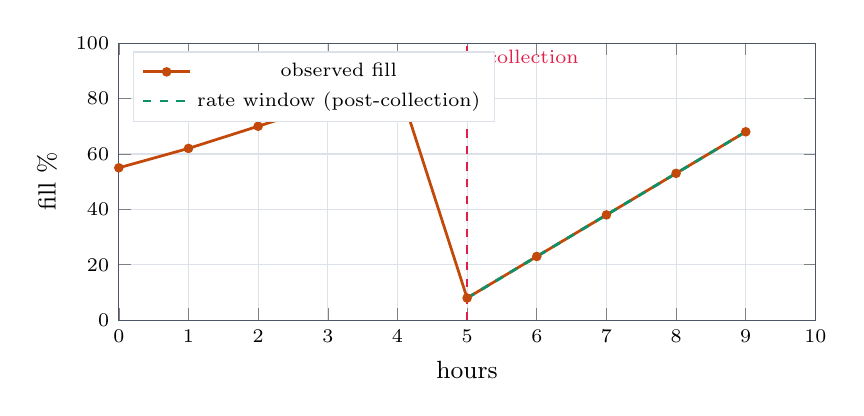
\begin{tikzpicture}
\begin{axis}[
  width=0.86\textwidth, height=5.1cm,
  xlabel={\small hours}, ylabel={\small fill \%},
  xmin=0, xmax=10, ymin=0, ymax=100,
  grid=major, grid style={rule},
  tick label style={font=\scriptsize},
  label style={font=\scriptsize},
  legend style={font=\scriptsize,at={(0.02,0.97)},anchor=north west,draw=rule},
  axis line style={inksoft}
]
\addplot[accent,line width=1pt,mark=*,mark size=1.2] coordinates {
  (0,55)(1,62)(2,70)(3,78)(4,86)(5,8)(6,23)(7,38)(8,53)(9,68)};
\addlegendentry{observed fill}
\addplot[low,dashed,line width=1pt] coordinates {(5,8)(9,68)};
\addlegendentry{rate window (post-collection)}
\draw[crit,line width=0.7pt,dashed] (axis cs:5,0) -- (axis cs:5,100);
\node[font=\scriptsize,color=crit,anchor=west] at (axis cs:5.15,95) {collection};
\end{axis}
\end{tikzpicture}
\caption{Fill history spanning a collection. Regressing across the cliff
would report a negative rate; the window opens at the collection, giving
$+15\,\%/\text{h}$.}
\end{figure}

\subsection{Verified output}

\begin{table}[h]
\centering\small
\begin{tabularx}{\textwidth}{lrlX}
\toprule
\textbf{Bin state} & \textbf{Score} & \textbf{Band} & \textbf{Reasons surfaced} \\
\midrule
Overflowing 96\,\%          & 76 & \textcolor{crit}{\textbf{Critical}} & 96\% full \\
Full 82\,\%, static         & 62 & \textcolor{high}{\textbf{High}}     & 82\% full \\
Offline 5\,h                & 55 & \textcolor{high}{\textbf{High}}     & Silent 5h ago \\
65\,\%, climbing fast       & 54 & \textcolor{high}{\textbf{High}}     & 65\% full; $\sim$2h to full \\
60\,\%, citizen report      & 53 & \textcolor{high}{\textbf{High}}     & 60\% full; Reported: Overflowing \\
65\,\%, static              & 40 & \textcolor{med}{\textbf{Medium}}    & 65\% full \\
92\,\% full, truck en route & 18 & \textcolor{low}{\textbf{Low}}       & EB-02 en route; 92\% full \\
97\,\%, under maintenance   & 15 & \textcolor{low}{\textbf{Low}}       & Under maintenance; 97\% full \\
\bottomrule
\end{tabularx}
\caption{Ranking over a constructed fleet.}
\end{table}

Two rows demonstrate the model. A bin at 65\,\% \emph{climbing fast}
scores 54 while an identical bin at 65\,\% \emph{sitting still} scores 40
--- by the time a truck arrives, the fast one is the overflow. And a
92\,\%-full bin with a truck already assigned falls to 18, because it is
not work anybody still needs to do.

\subsection{Urgency is not sufficient for dispatch}

A silent bin on a flat battery scores 68. It needs an engineer, not a
collection vehicle. The system therefore answers a second, independent
question --- is \emph{emptying} this bin the correct response? --- and
automatic dispatch requires both to be true:

\[
\text{dispatch} \iff (\text{score} \geq \theta) \;\wedge\; \text{needsCollection}
\]

where \texttt{needsCollection} is true when the bin is at or above the
full threshold, or projected full within the hour, or over capacity by
weight, or subject to an open overflow report. Offline and maintenance
bins therefore continue to raise alerts while never sending a truck.

% =====================================================================
\section{Fleet partitioning}

\subsection{Why the split precedes the route}

Which truck takes which bin determines far more of total fleet distance
than the stop order within any single run. Partitioning therefore happens
before any route is computed.

EcoBin uses sweep partitioning: order the bins by polar angle around the
depot, then walk that circle assigning contiguous angular wedges to each
truck until it is full. A wedge is naturally compact --- every bin in a
run lies in roughly the same direction from the depot, so no truck
crosses the city for a stop that another truck drove straight past.

\subsection{Searching the starting angle}

The classical sweep starts at an arbitrary angle, and that choice
matters as much as the ordering it produces: cutting the circle through a
tight cluster splits it between two trucks. EcoBin therefore evaluates
every stop as a candidate starting angle and keeps the cheapest resulting
partition. The cost is one straight-line tour estimate per rotation,
which is negligible at the size a real round runs to.

\begin{figure}[h]
\centering
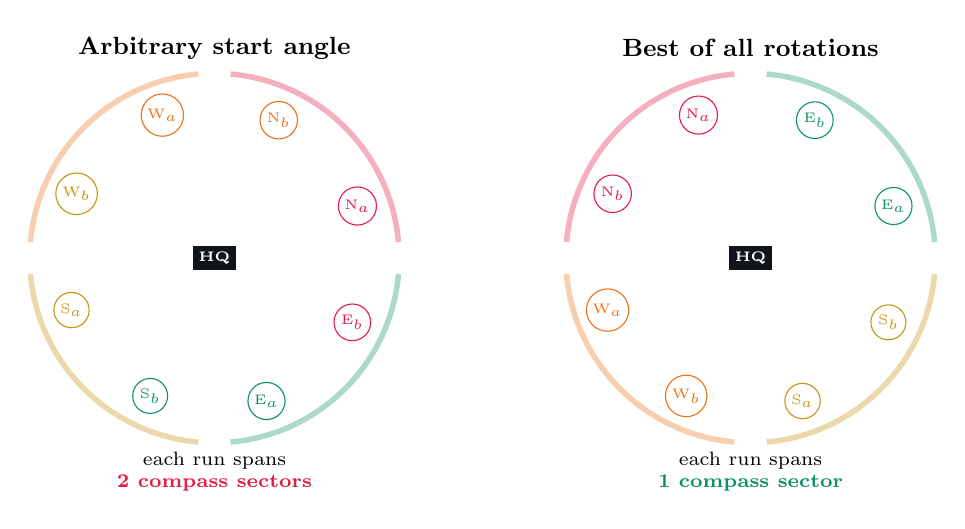
\begin{tikzpicture}[scale=0.92,
  bin/.style={circle,draw=ink,fill=white,inner sep=1.3pt,font=\tiny},
  dep/.style={rectangle,draw=ink,fill=ink,text=white,inner sep=2pt,font=\tiny\bfseries}
]
% ---- panel A : arbitrary start
\begin{scope}
\node[font=\small\bfseries] at (0,2.9) {Arbitrary start angle};
\node[dep] (d1) at (0,0) {HQ};
\foreach \a/\n/\c in {20/N$_a$/crit, 65/N$_b$/high, 110/W$_a$/high, 155/W$_b$/med,
                      200/S$_a$/med, 245/S$_b$/low, 290/E$_a$/low, 335/E$_b$/crit}
  \node[bin,draw=\c,text=\c] at (\a:2.1) {\n};
% wedge hints
\foreach \s/\c in {0/crit, 90/high, 180/med, 270/low}
  \draw[\c,line width=2pt,opacity=0.35] (\s+5:2.55) arc (\s+5:\s+85:2.55);
\node[font=\scriptsize,align=center] at (0,-2.95)
  {each run spans\\ \textcolor{crit}{\textbf{2 compass sectors}}};
\end{scope}
% ---- panel B : best rotation
\begin{scope}[xshift=7.4cm]
\node[font=\small\bfseries] at (0,2.9) {Best of all rotations};
\node[dep] (d2) at (0,0) {HQ};
\foreach \a/\n/\c in {20/E$_a$/low, 65/E$_b$/low, 110/N$_a$/crit, 155/N$_b$/crit,
                      200/W$_a$/high, 245/W$_b$/high, 290/S$_a$/med, 335/S$_b$/med}
  \node[bin,draw=\c,text=\c] at (\a:2.1) {\n};
\foreach \s/\c in {0/low, 90/crit, 180/high, 270/med}
  \draw[\c,line width=2pt,opacity=0.35] (\s+5:2.55) arc (\s+5:\s+85:2.55);
\node[font=\scriptsize,align=center] at (0,-2.95)
  {each run spans\\ \textcolor{low}{\textbf{1 compass sector}}};
\end{scope}
\end{tikzpicture}
\caption{Eight bins in four compass directions, four trucks at 200\,kg.
Colour denotes the assigned truck. Searching the starting angle collapses
every run onto a single sector.}
\end{figure}

\subsection{Capacity handling}

Capacity is respected where it is known. A truck with no stated capacity
receives an even share of the stops instead, so an unconfigured fleet
still partitions sensibly. Bins for which no truck has remaining capacity
are \emph{reported} to the operator rather than silently dropped.

Verified with 620\,kg of waste against 400\,kg of available trucks: two
runs planned within capacity, four bins explicitly deferred, zero trucks
over capacity.

% =====================================================================
\section{Route optimisation}

\subsection{Cost basis}

Stop order is optimised on real driving times obtained from the
OpenRouteService matrix endpoint, not straight-line distance. The
distinction is material: a river, a railway or a one-way system between
two bins that appear close together will make crow-flies ordering select
the wrong sequence.

Where no API key is configured, OSRM's public server supplies both the
matrix and the geometry without credentials; where neither is reachable,
the system falls back to great-circle distance and \emph{states in the
interface} that the ordering is approximate.

\subsection{Tour construction}

Nearest-neighbour builds an initial tour; 2-opt then repeatedly reverses
any segment that shortens it, until no improvement remains. The travelling
salesman problem admits no cheap proof of optimality, so this yields a
good tour rather than the best one --- but at the scale of a refuse round
it lands within a few percent, in microseconds, with no solver dependency.

\subsection{The double seed}

2-opt converges only to a \emph{local} optimum. Seeded from
nearest-neighbour alone, it can therefore return a tour worse than the
order it was handed. Measured over 300 randomised fleets, this occurred in
one case.

EcoBin runs 2-opt from two seeds --- the nearest-neighbour tour and the
input order --- and keeps whichever wins. Over the same 300 fleets, the
optimiser was worse than the input order in \textbf{zero} cases.

\begin{table}[h]
\centering\small
\begin{tabular}{lrr}
\toprule
\textbf{Seeding strategy} & \textbf{Worse than input} & \textbf{Trials} \\
\midrule
Nearest-neighbour only        & \textcolor{crit}{\textbf{1}} & 300 \\
Nearest-neighbour $+$ input   & \textcolor{low}{\textbf{0}}  & 300 \\
\bottomrule
\end{tabular}
\caption{A planner that claims a saving must never quietly cost more than
doing nothing.}
\end{table}

\subsection{Measured result}

\begin{figure}[h]
\centering
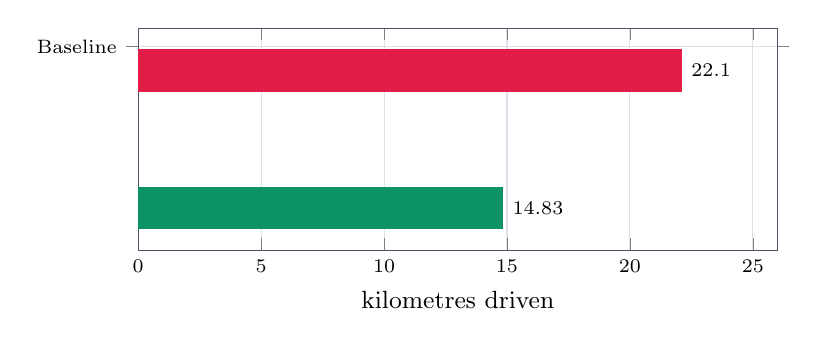
\begin{tikzpicture}
\begin{axis}[
  width=0.8\textwidth, height=4.4cm,
  xbar, xmin=0, xmax=26,
  xlabel={\small kilometres driven},
  symbolic y coords={Optimised,Baseline},
  ytick=data,
  nodes near coords, nodes near coords style={font=\scriptsize},
  tick label style={font=\scriptsize},
  label style={font=\scriptsize},
  bar width=15pt,
  grid=major, grid style={rule},
  axis line style={inksoft}
]
\addplot[fill=crit,draw=crit] coordinates {(22.10,Baseline)};
\addplot[fill=low,draw=low]  coordinates {(14.83,Optimised)};
\end{axis}
\end{tikzpicture}
\caption{Five bins, real Guwahati road network. Baseline is fullest-first
--- the order an operator drives without a planner.}
\end{figure}

\begin{table}[h]
\centering\small
\begin{tabular}{lrrrr}
\toprule
\textbf{Order} & \textbf{Distance} & \textbf{Diesel} & \textbf{\co{}} & \textbf{Saving} \\
\midrule
Fullest-first (baseline) & 22.10\,km & 7.89\,L & 21.2\,kg & --- \\
Optimised                & 14.83\,km & 5.30\,L & 14.2\,kg & \textbf{33\,\%} \\
\midrule
\multicolumn{4}{l}{\emph{Per run}} & 7.27\,km $\cdot$ 2.60\,L $\cdot$ \textbf{7.0\,kg \co{}} \\
\multicolumn{4}{l}{\emph{Annualised, three runs per day}} & \textbf{7.62\,t \co{}} \\
\bottomrule
\end{tabular}
\caption{Measured saving. Both halves computed on the same matrix, so the
comparison is like for like.}
\end{table}

\subsection{Geometry resolution}

\begin{table}[h]
\centering\small
\begin{tabular}{lrrl}
\toprule
\textbf{Source} & \textbf{Points} & \textbf{Distance} & \textbf{Result} \\
\midrule
Straight legs        & 7     & ---        & Crosses rivers and buildings \\
OSRM (keyless)       & 1{,}025 & 26.58\,km & Follows roads \\
OpenRouteService     & 725   & 26.25\,km  & Follows roads; identical stop order \\
\bottomrule
\end{tabular}
\caption{Same five stops. Both routing providers independently agree on
the optimal stop order.}
\end{table}

% =====================================================================
\section{Emissions model}

Carbon figures are easy to fabricate and hard to trust, so EcoBin's are
constructed to be auditable. Distance comes from the computed route, fuel
economy is an operator-supplied property of their own vehicle, and
exactly one constant is fixed:

\[
L = \frac{d_{\text{km}}}{\eta_{\text{km/L}}},
\qquad
m_{\co{}} = L \times 2.68\;\text{kg/L}
\]

Worked, for the optimised run above:

\[
\frac{14.83}{2.8} = 5.30\,\text{L},
\qquad
5.30 \times 2.68 = 14.2\,\text{kg }\co{}
\]

The constant $2.68\,\mathrm{kg/L}$ is a property of diesel fuel --- its
carbon content multiplied by the mass ratio of \co{} to carbon --- and
therefore does not vary by vehicle. The efficiency $\eta$ defaults to
$2.8\,\mathrm{km/L}$, within the 2.5--3 range typical of refuse
collection vehicles, and is configurable.

Critically, the reported saving is computed against the fullest-first
order \emph{on the same cost matrix}. Comparing a modelled optimised
figure against a real baseline, or vice versa, would produce a headline
number that is not a measurement of anything.

% =====================================================================
\section{Sensor integrity}

\subsection{The failure this addresses}

A load cell reads zero the instant anything lifts the load off it: a hand
on the lid, a sack being straightened, the sensor knocked during
maintenance. The bin remains full; only the reading collapsed.

Taken at face value, that zero removes the bin from the weight-based
terms of the ranking and causes the fleet weight total to understate
reality --- while the fill sensor continues to report 71\,\%. The two
sensors disagree, and the system must decide which to believe.

\subsection{Cross-validation rule}

A zero arriving while the bin still holds waste is treated as the
\emph{measurement} failing rather than the bin emptying. The last real
load is held until something actually empties the bin.

What releases the hold is a detected \emph{collection} --- which is
derived from the fill level dropping by at least 25\,\%. This is the
essential asymmetry: weight alone cannot establish that a bin was
emptied, because zero is precisely what a broken reading looks like. A
quarter drop in fill is something only an emptied bin does.

\begin{figure}[h]
\centering
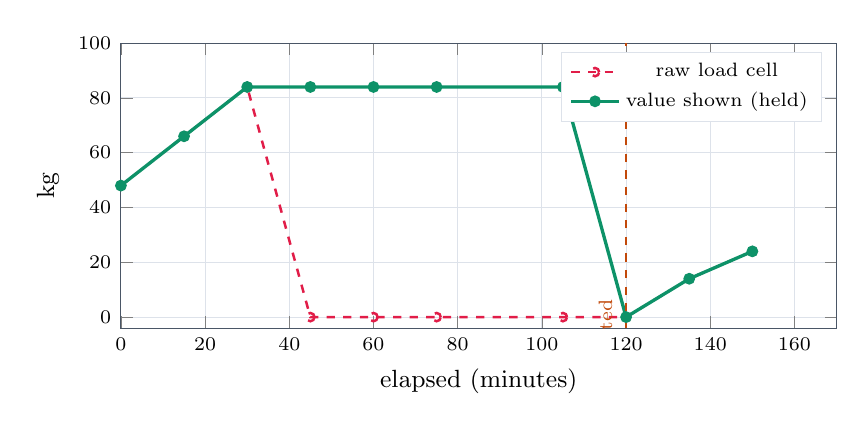
\begin{tikzpicture}
\begin{axis}[
  width=0.88\textwidth, height=5.2cm,
  xlabel={\small elapsed (minutes)}, ylabel={\small kg},
  xmin=0, xmax=170, ymin=-4, ymax=100,
  grid=major, grid style={rule},
  tick label style={font=\scriptsize},
  label style={font=\scriptsize},
  legend style={font=\scriptsize,at={(0.98,0.97)},anchor=north east,draw=rule},
  axis line style={inksoft}
]
\addplot[crit,line width=0.9pt,mark=o,mark size=1.5,dashed] coordinates {
  (0,48)(15,66)(30,84)(45,0)(60,0)(75,0)(105,0)(120,0)(135,14)(150,24)};
\addlegendentry{raw load cell}
\addplot[low,line width=1.2pt,mark=*,mark size=1.5] coordinates {
  (0,48)(15,66)(30,84)(45,84)(60,84)(75,84)(105,84)(120,0)(135,14)(150,24)};
\addlegendentry{value shown (held)}
\draw[accent,line width=0.7pt,dashed] (axis cs:120,-4) -- (axis cs:120,100);
\node[font=\scriptsize,color=accent,anchor=south east,rotate=90] at (axis cs:119,10) {collection detected};
\end{axis}
\end{tikzpicture}
\caption{Load lifted off at $t=45$; the bin is still 71\,\% full, so the
last real load is held. At $t=120$ the fill level drops by a quarter, a
collection is registered, and the hold releases to a true zero.}
\end{figure}

\subsection{Bounds on the rule}

The hold is narrow by construction, and every boundary was verified:

\begin{itemize}
  \item A bin with no load cell reports nothing --- never a fabricated zero.
  \item A bin reading zero since its last collection reports zero --- never held.
  \item A real reading is never overridden.
  \item A load recorded \emph{before} the last collection cannot leak forward
        into the current cycle; the lookback window closes at the collection.
\end{itemize}

Where a held value is displayed the interface says so explicitly. The
readings chart deliberately continues to plot the raw dip to zero: it is
the record of what the sensor reported, and smoothing history is a
separate decision from determining what the bin weighs now.

\subsection{The governing principle}

Throughout the codebase, a measurement the device never sent remains
\texttt{null} and renders as a dash. There is no zero-filling, no silent
substitution of last-known values, and no invented averages. The load-cell
hold above is the single deliberate exception, and it is labelled
everywhere it appears.

% =====================================================================
\section{Automation and dispatch}

\subsection{Decision flow}

\begin{figure}[h]
\centering
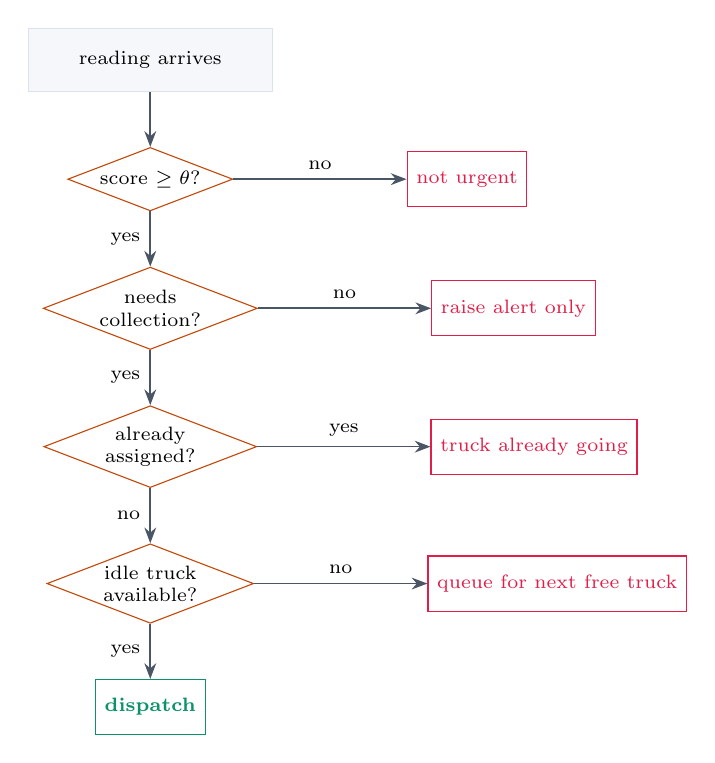
\begin{tikzpicture}[
  node distance=7mm and 9mm,
  box/.style={draw=rule,fill=wash,minimum height=8mm,minimum width=3.1cm,
              align=center,font=\scriptsize},
  dec/.style={draw=accent,fill=white,diamond,aspect=2.6,inner sep=1pt,
              align=center,font=\scriptsize},
  no/.style={draw=crit,fill=white,minimum height=7mm,align=center,font=\scriptsize,text=crit},
  yes/.style={draw=low,fill=white,minimum height=7mm,align=center,font=\scriptsize,text=low},
  ar/.style={-{Stealth[length=2mm]},draw=inksoft,line width=0.6pt,font=\scriptsize}
]
\node[box] (r) {reading arrives};
\node[dec,below=of r] (s) {score $\geq \theta$?};
\node[dec,below=of s] (n) {needs\\collection?};
\node[dec,below=of n] (a) {already\\assigned?};
\node[dec,below=of a] (t) {idle truck\\available?};
\node[yes,below=of t] (go) {\textbf{dispatch}};

\node[no,right=22mm of s] (s2) {not urgent};
\node[no,right=22mm of n] (n2) {raise alert only};
\node[no,right=22mm of a] (a2) {truck already going};
\node[no,right=22mm of t] (t2) {queue for next free truck};

\draw[ar] (r) -- (s);
\draw[ar] (s) -- node[left]{yes} (n);
\draw[ar] (n) -- node[left]{yes} (a);
\draw[ar] (a) -- node[left]{no} (t);
\draw[ar] (t) -- node[left]{yes} (go);
\draw[ar] (s) -- node[above]{no} (s2);
\draw[ar] (n) -- node[above]{no} (n2);
\draw[ar] (a) -- node[above]{yes} (a2);
\draw[ar] (t) -- node[above]{no} (t2);
\end{tikzpicture}
\caption{Automatic dispatch. Every branch was verified against a
constructed fleet.}
\end{figure}

\subsection{Verified guards}

\begin{table}[h]
\centering\small
\begin{tabularx}{\textwidth}{Xl}
\toprule
\textbf{Scenario} & \textbf{Outcome} \\
\midrule
Two idle trucks, one bin over threshold          & Dispatched; best-fit truck by capacity \\
Offline bin scoring 68                           & Not dispatched --- needs an engineer \\
No idle trucks                                   & Nothing dispatched; bin stays queued \\
Operator cancelled this bin                      & Held back for a cooldown, not overruled \\
Bin already assigned                             & No second truck sent \\
120\,kg load; 300\,kg and 900\,kg trucks free    & Smallest that fits; large truck kept free \\
Bin full across five consecutive readings        & Dispatched exactly once \\
\bottomrule
\end{tabularx}
\caption{Dispatch guards.}
\end{table}

\subsection{Idempotence across a full episode}

A workflow observing ThingSpeak reports a bin as full for as long as it
\emph{is} full --- every reading until a truck empties it. Each such
report carries a distinct command identity. Without a guard, the same bin
would be dispatched on every poll, reassigning it and pulling a second
truck off its own work.

\begin{table}[h]
\centering\small
\begin{tabular}{llrl}
\toprule
\textbf{Reading} & \textbf{Fill} & \textbf{Commands} & \textbf{Action} \\
\midrule
1 & 62\,\% & 0 & --- \\
2 & 84\,\% & 1 & \textcolor{low}{\textbf{dispatched}} \\
3 & 88\,\% & 1 & no action (already assigned) \\
4 & 91\,\% & 1 & no action \\
5 & 95\,\% & 1 & no action \\
6 & \phantom{0}6\,\% & 0 & collected; assignment cleared \\
7 & 83\,\% & 1 & \textcolor{low}{\textbf{dispatched}} \\
\midrule
\multicolumn{3}{l}{\textbf{Total dispatches}} & \textbf{2} --- one per full episode \\
\bottomrule
\end{tabular}
\caption{This property allows the n8n workflow to remain stateless: it
reports every bin currently over threshold, without tracking what it has
already said.}
\end{table}

\subsection{Fleet execution}

Once dispatched, runs execute on the map with per-truck lanes, heading-
oriented markers and live arrival estimates.

\begin{table}[h]
\centering\small
\begin{tabular}{llrl}
\toprule
\textbf{Phase} & \textbf{Detail} & & \\
\midrule
Split   & TR-01 & 278\,kg / 300\,kg & Hospital, Market, Terminus, Riverside \\
        & TR-02 & 119\,kg / 300\,kg & Station Road \\
\midrule
Plan    & TR-01 & 12.18\,km, 29\,min & Depot $\rightarrow$ Riverside $\rightarrow$ Terminus $\rightarrow$ Market $\rightarrow$ Hospital $\rightarrow$ Depot \\
\midrule
\multirow{5}{*}{Drive}
        & $t$+20\,s & 23\,\% & arrived Riverside Park \\
        & $t$+40\,s & 46\,\% & arrived Bus Terminus \\
        & $t$+50\,s & 57\,\% & arrived Market Complex \\
        & $t$+75\,s & 86\,\% & arrived Civil Hospital \\
        & $t$+90\,s & 100\,\% & returned to depot; 4 of 4 collected \\
\midrule
Effect  & Station Road & 82\,\% $\rightarrow$ 2\,\% & collection detected by the pipeline \\
\bottomrule
\end{tabular}
\caption{Complete lifecycle from one command. Reaching a bin empties it,
producing a genuine cliff in that bin's history --- so the system's own
collection detection fires exactly as it would on physical hardware.}
\end{table}

Route lanes are coloured by the urgency of a run's \emph{remaining}
stops, on the same scale the bins use, so a red lane and a red bin badge
carry identical meaning and a run cools from red toward green as it is
worked. The banding is weighted by the proportion of stops over the full
threshold: a route of four bins all in the eighties reads critical, while
one critical bin among three empty ones does not --- that is a route with
one urgent stop, not an urgent route.

% =====================================================================
\section{Implementation}

\subsection{Stack}

React~19 with Vite~8. Leaflet over OpenStreetMap tiles for the operations
map; Recharts for time series. Firebase Firestore for shared state and
command delivery. The production output is a static bundle deployable to
any host --- there is no EcoBin server component.

\begin{table}[h]
\centering\small
\begin{tabularx}{\textwidth}{lrX}
\toprule
\textbf{Module} & \textbf{Lines} & \textbf{Contents} \\
\midrule
\texttt{components/} & 4{,}994 & Dashboard panels, operations map, pages, citizen app \\
\texttt{context/}    & 1{,}215 & State, auto-dispatch, run planning, fleet simulation, n8n \\
\texttt{services/}   & \phantom{0}957 & ThingSpeak, routing and optimisation, partitioning, Firebase \\
\texttt{lib/}        & \phantom{0}755 & Telemetry parsing, priority scoring, emissions, simulation \\
\texttt{hooks/}      & \phantom{0}191 & Polling; shared state with local fallback \\
\texttt{config/}     & \phantom{0}182 & Runtime settings layered over environment and storage \\
\midrule
\textbf{Total}       & \textbf{8{,}441} & across 37 files \\
\bottomrule
\end{tabularx}
\caption{Source layout.}
\end{table}

\subsection{External services}

ThingSpeak provides telemetry. OpenRouteService provides the driving-time
matrix, geocoding and route geometry, with OSRM as a keyless fallback.
n8n makes the dispatch decision. Firestore delivers commands and shares
operator state between dashboards.

\subsection{Operator surface}

\begin{itemize}
  \item \textbf{Dashboard} --- live weight and fleet indicators, operations
        map with routes and moving trucks, priority list, selected-bin
        telemetry, alerts, collection progress.
  \item \textbf{Map} --- full operations view with numbered stops, depot,
        per-run lanes and live tracking cards.
  \item \textbf{Bins, Collection, Trucks, Alerts, Reports} --- operational registers.
  \item \textbf{Segregation} --- waste-category breakdown from an on-device
        classifier field.
  \item \textbf{Citizen app} --- public reporting surface; a report raises the
        subject bin's priority by 18 points.
  \item \textbf{Settings} --- channels and field mapping, thresholds, depot,
        fuel economy, auto-dispatch, n8n control, simulation.
\end{itemize}

% =====================================================================
\section{Verification}

Every algorithm described above was executed against constructed fleets
and live APIs before being trusted. That process located seven defects,
several of which read as correct on the page.

\begin{table}[h]
\centering\small
\begin{tabularx}{\textwidth}{lX}
\toprule
\textbf{Defect} & \textbf{Root cause} \\
\midrule
Matrix API never answered &
OpenRouteService names the parameter \texttt{locations} for the matrix
endpoint and \texttt{coordinates} for directions. The resulting HTTP 400
is indistinguishable from every other reason to fall back, so all routes
were silently ordered by the fallback provider. \\
\addlinespace
Fleet drained to nothing &
A detected collection cleared the assignment but never returned the truck
to idle. Invisible while dispatch was manual and status was editable. \\
\addlinespace
Bins stuck as assigned &
A nearly empty bin never drops far enough to register a collection, so its
assignment never cleared when the run completed. \\
\addlinespace
Markers rebuilt at 1\,Hz &
Supplying a new icon object makes Leaflet discard and rebuild the element.
A CSS transition cannot animate an element that did not previously exist,
so smooth movement never occurred and pulse animations restarted each second. \\
\addlinespace
Optimiser could lose &
2-opt from a single seed converges to a local optimum, occasionally worse
than the input order. \\
\addlinespace
Working API key ignored &
A blank key persisted to local storage shadowed the configured one,
because stored values take precedence over defaults. \\
\addlinespace
Repeated dispatch &
A full bin remains full across many readings, each carrying a new command
identity. \\
\bottomrule
\end{tabularx}
\caption{Defects located by verification rather than by inspection.}
\end{table}

Priority scoring was additionally consolidated from five independent call
sites into a single computation per telemetry update. A map lookup is
approximately 33 times cheaper than a rescore, and the cost now scales
with the data rather than with a one-second animation clock.

% =====================================================================
\section{Scope: real and simulated}

Stated explicitly, because a demonstration that overstates itself is
worth less than one that does not.

\subsection{Real}

\begin{itemize}
  \item Live ThingSpeak telemetry from a physical bin --- fill level and
        weight on a production channel.
  \item Road routing, driving-time matrices and geometry from
        OpenRouteService and OSRM against the real Guwahati road network.
  \item Firestore as deployed infrastructure; state sharing and command
        delivery both verified against the live project.
  \item Every algorithm --- ranking, partitioning, optimisation, emissions,
        sensor fusion --- operating on whatever data it is given.
\end{itemize}

\subsection{Simulated}

\begin{itemize}
  \item Five additional bins, so that routing and ranking have a fleet to
        operate on before further hardware exists. They follow a sawtooth
        that fills and is collected on cycles dividing evenly into a day,
        and are badged \textsc{sim} everywhere they appear.
  \item Truck movement. Distances, stop order, fuel and \co{} are real;
        playback is accelerated because a real round occupies most of an hour.
  \item Trucks carry no GPS, so vehicle selection is by capacity fit rather
        than proximity. The interface says ``dispatch'', never ``nearest'',
        because the available data cannot support that claim.
\end{itemize}

A single setting removes the simulation entirely, after which the
dashboard shows only physical bins. No stage of the pipeline treats a
simulated bin differently from a real one.

% =====================================================================
\section{Future work}

\begin{enumerate}
  \item \textbf{Driver application.} The run is planned and tracked, but
        reaches the driver only through the operator. A stop list with
        tap-to-confirm closes the final gap and removes the dependence on
        fill-drop detection for run completion.
  \item \textbf{Hardened Firestore rules.} Currently open for demonstration.
        Service-account authentication for n8n and per-operator rules are
        required before any real deployment.
  \item \textbf{Predictive scheduling.} Fill rate is already computed;
        projecting each bin forward converts tomorrow's round into
        something planned this afternoon rather than reacted to at dawn.
  \item \textbf{Vehicle telematics.} GPS on trucks makes proximity dispatch
        honest and converts simulated movement into observed movement.
  \item \textbf{Multi-depot partitioning.} The sweep assumes a single depot;
        a city-scale fleet needs the split to consider several.
\end{enumerate}

% =====================================================================
\section{Conclusion}

EcoBin demonstrates that the value in a sensor-instrumented waste system
lies not in the sensors but in the decisions taken on their output. The
same five bins, the same telemetry and the same fleet produce a 22.10\,km
round under a naive fullest-first policy and a 14.83\,km round under
geographic optimisation --- a 33\,\% reduction, 7.0\,kg of \co{} per run,
and approximately 7.6 tonnes annually at three runs per day.

The engineering emphasis throughout has been on decisions that remain
defensible under examination: an optimiser that cannot lose to doing
nothing, an emissions figure whose arithmetic is exposed rather than
asserted, a dispatch rule that distinguishes urgency from appropriateness,
and a sensor-fusion rule that prefers to say ``held'' rather than report a
number it does not believe.

\vfill
\begin{center}\small
\textcolor{inksoft}{Every figure in this report was produced by executing the system. None are estimated.}
\end{center}

\end{document}
